\section{Combining Fine-Tuning with Inference-Time Techniques}\label{sec:fine_tuning} 

\begin{figure}[!ht]
\centering
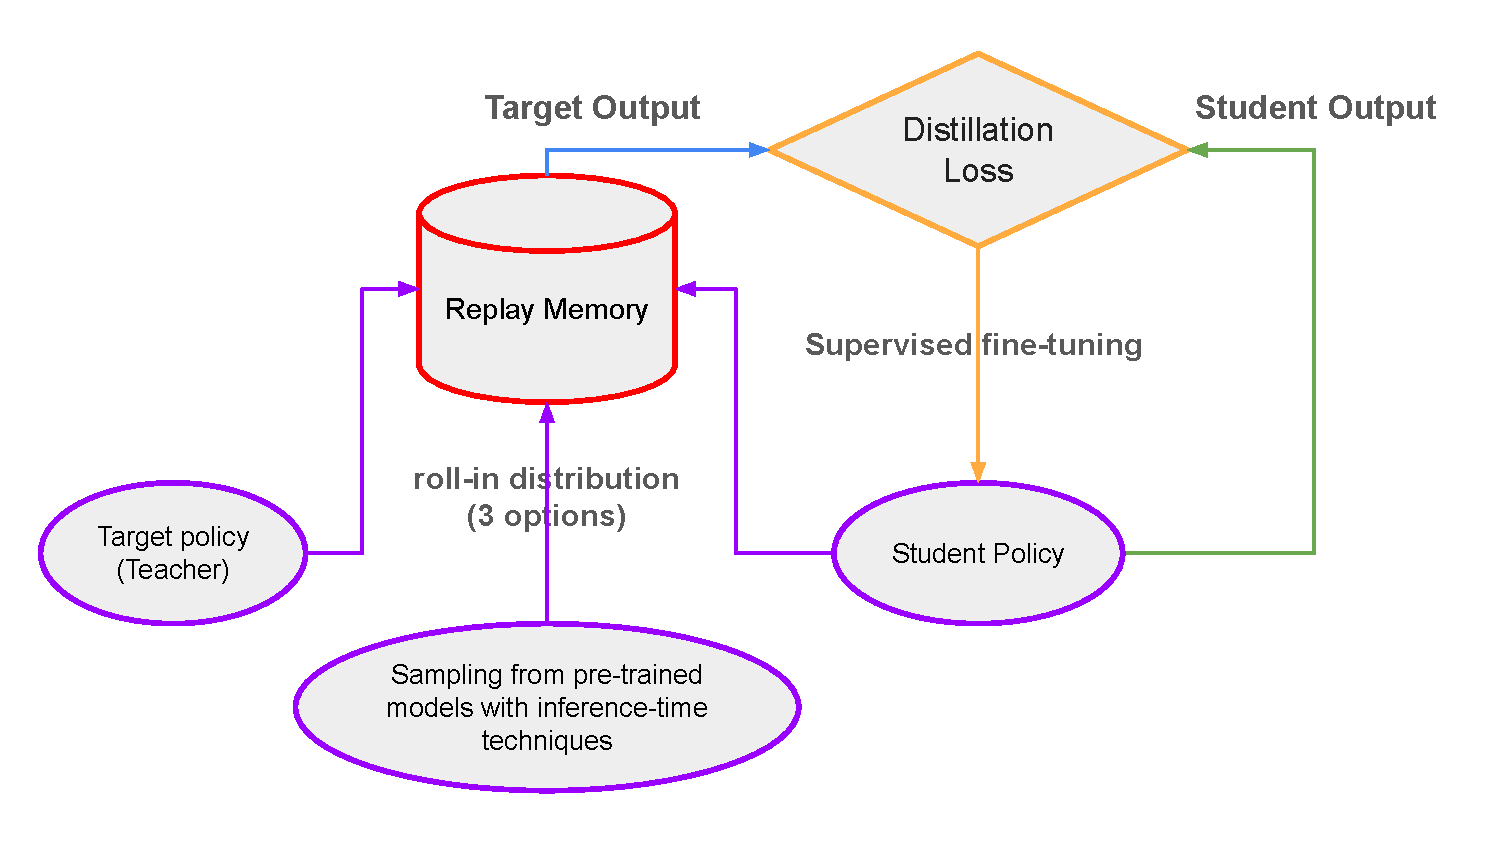
\includegraphics[width=0.9\textwidth]{images/distillation.pdf}
  \caption{Visualization of policy distillation that leverages inference-time techniques in fine-tuning.
  }
\label{fig:distil}
\end{figure}




While the inference-time techniques discussed so far have proven effective, a potential bottleneck lies in the extended inference time required to generate samples. For instance, in derivative-free guidance (\pref{sec:derivative_free}), value functions must be evaluated at each time step. Similarly, in derivative-based guidance (\pref{sec:derivative}), the derivatives of value functions need to be computed.


To mitigate this issue, we outline fine-tuning strategies to accelerate inference time. Our primary approach involves \emph{policy distillation}, a widely adopted technique in RL \citep{rusu2015policy,czarnecki2019distilling}. We also emphasize its connection to RL-based fine-tuning in diffusion models, which is summarized in \citet{uehara2024understanding}. Finally, we briefly review methods for minimizing inference time in the context of pure diffusion models (i.e., without alignment considerations), which can be applied following policy distillation.

Before delving into the details of policy distillation, we first emphasize the differences between inference-time techniques and standard post-training methods in diffusion models, such as classifier-free fine-tuning and RL-based fine-tuning.


\subsection{Comparison with Standard Post-Training Methods}


We compare inference-time techniques with several alternative post-training approaches that achieve the same goal—generating natural-like designs with high functionality.

\subsubsection{Classifier-Free Fine-Tuning}\label{sec:classfier_free}

Classifier-free guidance \citep{ho2022classifier} aims to directly model the target conditional distribution $p^{(\alpha)}(x \mid y)$ by leveraging an unconditional model and adjusting the guidance scale. This method can be applied to fine-tuning when we have a pre-trained model, which characterizes $p^{\pre}\in \Delta(\Xcal)$, and a reward (or classifier) as follows: 

\begin{enumerate} 
\item  Construct a dataset $\mathcal{D} = \{x_i, y_i\}$ where $x \sim p^{\pre}(x)$ and $y = r(x)$ (or $y \sim p(y \mid x)$). If an alternative dataset $\mathcal{D}'$ is available, it can be used to augment the dataset.
\item %
{ Perform classifier-free guidance by fine-tuning the pre-trained model with the constructed dataset. Here, we augment the model with additional parameters to integrate new conditioning $y$, as implemented in ControlNet \citep{zhang2023adding}.} 
\item After fine-tuning, if the objective is conditioning, generate samples conditioned on the target $y$. If the objective is alignment, condition on high values of $y$.
\end{enumerate}

The performance of this approach is highly dependent on the amount of data available in the first step. Specifically, when working with known reward feedback (e.g., inverse problems or non-differentiable simulation-based feedback), this method can be extremely sample-inefficient, as the feedback must be translated into a large dataset that effectively captures the reward signal. Furthermore, this dataset must be transformed into models with additional parameters, which significantly increases computational requirements during both training and inference.


Furthermore, this sample inefficiency becomes more severe when the pre-trained models are conditional diffusion models $p(x \mid c): \mathcal{C} \to \Delta(\mathcal{X})$, and multiple classifiers or rewards $r_1: \mathcal{X} \to \mathbb{R}, \dots, r_M: \mathcal{X} \to \mathbb{R}$ need to be optimized. In such cases, it is necessary to construct pairs of the form $\{c, x, r_1(x), \dots, r_M(x)\}$, rather than separate datasets $\{x, r_i(x)\}$ for each reward function, which requires considerable effort. By contrast, the inference-time techniques reviewed in this work do not involve inefficient data augmentation steps or potentially challenging training processes. 


{ Finally, it is worth noting that the inference-time techniques introduced so far could assist in classifier-free fine-tuning during the data augmentation step. In this way, classifier-free fine-tuning and inference-time techniques can be integrated in a complementary manner.} 

\subsubsection{RL-Based Fine-Tuning}

RL-based fine-tuning has been employed to optimize rewards by embedding diffusion models into Markov Decision Processes (MDPs). Seminal works have been proposed using policy gradient methods such as PPO \citep{fan2023dpok,black2023training}. However, given that many important reward functions in computer vision are differentiable, recent state-of-the-art methods focus on variants of direct backpropagation approaches \citep{clark2023directly,prabhudesai2023aligning}.

In molecular design, RL-based fine-tuning presents additional challenges, as most useful feedback is highly non-differentiable. In many cases, policy gradient methods remain necessary over direct backpropagation. However, based on the authors' experience, optimizing such reward functions through policy gradient-based fine-tuning is still difficult, as the landscapes of reward functions are highly complicated. 

In contrast, the inference-time techniques introduced in this review are straightforward to implement, as many of them are not only fine-tuning-free but also training-free. As will be discussed in \pref{sec:foundation}, while both RL-based and inference-time methods ideally aim to reach the same optimal policy, inference-time techniques are generally more stable for alignment. This is because they directly sample from the optimal target policy by guiding individual particles (samples) without altering the underlying diffusion models. On the other hand, RL-based fine-tuning must guide the entire generative model, which encapsulates the information of all generated samples. As a result, RL-based fine-tuning is significantly more challenging. Consequently, inference-time techniques are more effective across various domains, including molecular design, even when reward feedback is highly non-differentiable, as demonstrated in \citet{li2024derivative}.

Lastly, we highlight that inference-time methods can also enhance fine-tuning through policy distillation. We compare this hybrid approach with RL-based fine-tuning in more detail in \pref{sec:fine_tuning}.



\subsection{Policy Distillation}\label{sec:policy_distil}


So far, we have discussed two standard techniques for post-training. In this subsection, we introduce an alternative approach: policy distillation for fine-tuning, leveraging the inference-time techniques presented earlier. The key idea is to fine-tune diffusion models so that the fine-tuned models replicate the trajectories generated by the inference-time technique. Through the iterative application of this process, the fine-tuned models can gradually improve, as illustrated in \pref{fig:distil}.

{ Hereafter, we refer to the inference-time techniques (e.g., SMC-based guidance, value-based importance sampling, and classifier guidance targeting $p^{\star}_{t-1}:\Xcal \to \Delta(\Xcal)$) as teacher policies. The policies being fine-tuned, represented as $p_{t-1}(\cdot \mid \cdot; \theta):\Xcal \to \Delta(\Xcal)$, are referred to as student policies, adopting the terminology from RL \citep{czarnecki2019distilling}.  } 

Algorithms in this section are summarized in the following master formulation. 


\begin{AIbox}{Master Formulation}
Introducing a roll-in distribution $u_t \in \Delta(\Xcal)$, and an $f$-divergence between teacher and student policies at time $t$, the policy distillation is formulated as an iterative algorithm using the update: 
\begin{align*}
    \theta^{\mathrm{new}} \leftarrow \theta^{\mathrm{old}}  - \gamma \sum_{t=T+1}^1 \EE_{x_t \sim u_t}[ \nabla_{\theta} 
 f(p^{\star}_{t-1}(\cdot \mid x_t) \|p_{t-1}(\cdot \mid x_t;\theta) )]|_{\theta^{\mathrm{old}}}, 
\end{align*}
where $\gamma$ is a learning rate. 
\end{AIbox}
Hereafter, we elaborate on two critical points. 






\subsubsection{Choice of Roll-In Distributions} 

The selection of the roll-in distribution is critical, as optimizing the empirical objective with function approximation ensures low error only within the distribution's support. Potential choices include (1) the teacher policy, (2) the student policy (the one being optimized), and (3) data recycling via forward processes. These distributions can also be mixed. We will explore these options in greater detail.

\paragraph{Teacher Policy.} This approach is often called offline policy distillation, as the roll-in distribution remains fixed throughout fine-tuning. 
Since this corresponds to the target policy, it is always a reasonable choice. However, it could have a distributional shift \citep{ross2010efficient}: during fine-tuning, the model encounters states it has not previously observed yet, which can result in poor performance.

\paragraph{Student Policy.} This approach is often referred to as online policy distillation, as roll-in samples are collected in an online manner. In the RL context, it is employed in the well-known algorithm DAgger \citep{ross2011reduction}. This method mitigates the distributional shift issue mentioned earlier by aligning the training distribution with the distribution induced by the current student policy. In practice, it can be beneficial to mix distributions induced by both teacher and student policies, as demonstrated in \citet{ross2011reduction,sun2017deeply,chang2023learning}.

\paragraph{Data Recycling via Forward Processes.}

In both scenarios described above (using teacher or student policies as roll-in distributions), the roll-in distributions are generated by sampling from $x_T$ to $x_t$. However, employing teacher policies as roll-in distributions can be computationally expensive.

To mitigate this inefficiency, an alternative approach leverages the forward process in pre-trained diffusion models, sampling from $x_0$ to $x_t$, which is computationally faster than sampling from 
 $x_T$ to $x_t$. Specifically, assume we have access to the dataset used to train the pre-trained models or data obtained at time $0$ through inference-time techniques.  Let this dataset be denoted as $\Dcal =\{x^i_0\}_{i=1}^N$.  Using this dataset $\Dcal$, we can generate roll-in distributions by sampling $x_t$ from the forward policies of the pre-trained models, starting from $x_0$. Consequently, the loss function becomes:
\begin{align}
\label{eq:loss_forward_roll_in_distribution}
    \frac{1}{|\Dcal| }\sum_{i=1}^{|\Dcal|} \sum_{t=T+1}^1  \EE_{x_t \sim q_t(\cdot \mid x^i_0) }\left [f(p^{\star}_{t-1}(\cdot \mid x_t) \|p_{t-1}(\cdot \mid x_t;\theta) )\right ], 
\end{align}
where $q_t(\cdot|x^i_0)$ represents the distribution induced by the forward policies of the pre-trained models from $x_0$ to $x_t$.




\subsubsection{Choice of Divergence}

The choice of divergence is critical. Common options include KL divergence and inverse KL divergence.

\paragraph{KL Divergence.} In this case, the gradient is 
\begin{align}\label{eq:KL_appraoch}
 \sum_{t=T+1}^1 \EE_{x_t\sim u_t} \left[ \nabla_{\theta} \KL(p^{\star}_{t-1}(\cdot|x_t) \| p_{t-1}(\cdot \mid x_t;\theta))   \right]|_{\theta^{\mathrm{old}}}. 
\end{align}
This can be further simplified to:
\begin{align*}
 \sum_{t=T+1}^1 \EE_{x_t\sim u_t, x_{t-1}\sim p^{\star}(x_t) } \left[\nabla_{\theta}  \log p_{t-1}(x_{t-1} \mid x_t;\theta)  \right]|_{\theta^{\mathrm{old}}}. 
\end{align*} 
When using marginal distributions induced by teacher policies as roll-in distributions, this approach is particularly intuitive, as it minimizes the KL divergence between the distributions induced by the teacher and student policies. In generative models, KL divergence is commonly employed since it effectively covers the target distribution (i.e., it is less mode-seeking but more conservative).

\paragraph{Inverse KL Divergence.}

In this case, the gradient is 
\begin{align}
    \sum_{t=T+1}^1 \EE_{x_t\sim u_t} \left[\nabla_{\theta} \KL(p_{t-1}(\cdot \mid x_t;\theta) \| p^{\star}_{t-1}(\cdot|x_t))   \right]|_{\theta^{\mathrm{old}}}.  \label{eq:inverse_KL}
\end{align}
Substituting the form of the optimal policy $p^{\star}_{t-1}$, it simplifies to:
\begin{align}
  \sum_{t=T}^0  \EE_{x_t \sim u_t} \left[ \nabla_{\theta}\EE_{x_{t-1}\sim p_{t-1}(x_t;\theta) } \left [ \log p_{t-1}(x_{t-1}|x_t;\theta) -\log p^{\pre}_{t-1}(x_{t-1}\mid x_t) -\frac{v_{t-1}(x_{t-1})}{\alpha} + \frac{v_{t}(x_{t})}{\alpha}    |x_t \right] \right]. \label{eq:all_form}
\end{align}

This method is inherently more mode-seeking. While this property can be disadvantageous when the goal is to cover diverse regions, it becomes beneficial when the primary focus is on optimization without prioritizing diversity.









\subsection{Relation to RL-Based Fine-Tuning}

In this section, we establish the connection between the policy distillation approach discussed earlier and existing RL-based fine-tuning methods, which are summarized in \citet{uehara2024understanding}. 

\subsubsection{Value-Weighted MLE (Reward-Weighted MLE)}

First, we relate the KL-based distillation approach to value-weighted maximum likelihood estimation (MLE). Recall that $p^{\star}_{t-1}$ is a value-tilted policy proportional to $p^{\pre}_{t-1}(\cdot \mid x_{t-1})\exp(v_{t-1}(\cdot))$. When the divergence function $f$ is the KL divergence, the gradient formulation (\ref{eq:KL_appraoch}) becomes:
\begin{align*}
      \sum_{t=T+1}^1 \EE_{x_t \sim u_t}\left [ \nabla_{\theta} \EE_{ x_{t-1}\sim p^{\pre}(x_t)}\left [\exp\left ( \frac{v_{t-1}(x_{t-1})}{\alpha} \right)\log p_{t-1}(x_{t-1}|x_t;\theta) \right] \right ]. 
\end{align*}

This formulation is known in the RL literature as value-weighted MLE \citep{peng2019advantage,peters2010relative}. In the context of fine-tuning diffusion models, it reduces to the objective function defined in \citet[Algorithm 3]{uehara2024understanding}. 

\subsubsection{Path Consistency Learning (loss used in Gflownets)}

Next, recall the soft-Bellman equation:
\begin{align*}
    \int p^{\pre}_{t-1}(x|x_{t})\exp(v_{t-1}(x)/\alpha)dx = \exp(v_{t}(x_t)/\alpha). 
\end{align*}
Then, by taking the logarithm of the optimal policy
\begin{align*}
    p^{\pre}_{t-1}(\cdot|x_{t})= \exp(v_{t-1}(\cdot)/\alpha)p^{\pre}_{t-1}(x|x_{t})/ \exp(v_{t}(x_t)/\alpha), 
\end{align*}
this reduces to 
\begin{align*}
     \log p^{\star}_{t-1}(x_{t-1}|x_t) -\log p^{\pre}_{t-1}(x_{t-1}\mid x_t) -\frac{v_{t-1}(x_{t-1})}{\alpha} + \frac{v_{t}(x_{t})}{\alpha}=0. 
\end{align*}
From the above equation, the optimal policy is estimated by minimizing the following objective: 
\begin{align*}
     \sum_{t=T+1}^1  \EE_{(x_{t-1},x_t) \sim u_t} \left[\left \| \log p_{t-1}(x_{t-1}|x_t;\theta) -\log p^{\pre}_{t-1}(x_{t-1}\mid x_t) -\frac{v_{t-1}(x_{t-1})}{\alpha} + \frac{v_{t}(x_{t})}{\alpha}   \right \|^2 \right]. 
\end{align*}
This objective aligns with the path-consistency RL objective commonly discussed in the RL literature \citep{nachum2017bridging}. In RL-based fine-tuning, it reduces to the objective defined in \citet[Algorithm 5]{uehara2024understanding}. Note several improved variants have also been proposed in \citet{rector2024steering,venkatraman2024amortizing}.

The above is closely related to the inverse KL divergence objective \eqref{eq:all_form}. However, PCL is generally regarded as more stable, as the expectation in \eqref{eq:all_form} depends on the parameter being optimized.

\subsubsection{PPO and Direct Backpropagation}

In the RL-based fine-tuning literature~\citep{fan2023dpok,black2023training}, the standard objective is:
\begin{align}\label{eq:PPO}
   \argmax_{\theta} \EE_{\{p^{\theta}_t\}_{t=T+1}^1} \left[r(x_0)- \alpha \sum_{t=T+1}^1 \KL(p_{t-1}(\cdot|x_t;\theta) \| p^{\pre}_{t-1}(\cdot|x_t))   \right], 
\end{align}
where the expectation is taken with respect to $p^{\theta}$. As demonstrated in \citet[Theorem 1]{uehara2024bridging}, the policy that maximizes the above (in the absence of optimization or function approximation errors) is equal to the optimal policy we aim to target during inference, i.e., $p^{\star}_{t-1}$ in \eqref{eq:optimal_policy}. 

While solving the optimization problem in \eqref{eq:PPO} is non-trivial in practice, policy gradient methods (or their variants) can be employed \citep{black2023training,fan2023dpok}. Then, ignoring KL terms to simplify the notation here, the optimization step becomes 
\begin{align}\label{eq:PPO2}
    \theta^{\mathrm{old}}  +  \gamma \EE_{\{p^{\theta^{\mathrm{old}}}_t\}_{t=T+1}^1} \left[r(x_0) \sum_{t=T+1}^1 \frac{\nabla_{\theta} p_{t-1}(\cdot \mid x_{t};\theta )}{p_{t-1}(\cdot \mid x_{t};\theta^{\mathrm{old}})}    \right]|_{\theta^{\mathrm{old}}}.
\end{align}
Furthermore, when the reward function is differentiable, direct backpropagation becomes a feasible approach \citep{clark2023directly,prabhudesai2023aligning}. 

It is worthwhile to note the above objective function in \eqref{eq:PPO} is essentially equivalent to the inverse KL divergence: 
\begin{align*}
   \sum_{t=T+1}^1  \EE_{\{p^{\theta}_t\}_{t=T+1}^1}[\mathrm{KL}(p_{t-1}(\cdot\mid x_{t-1};\theta)\|p^{\star}_{t-1}(\cdot\mid x_{t-1}))  ]. 
\end{align*}
This is seen by 
{\begin{align*}
    & - \alpha \sum_{t=T+1}^1 \EE_{\{p^{\theta}_t\}_{t=T+1}^1}[\mathrm{KL}(p_{t-1}(\cdot\mid x_{t-1};\theta)\|p^{\star}_{t-1}(\cdot\mid x_{t-1}))  ]\\
    &=- \alpha \sum_{t=T+1}^1 \EE_{\{p^{\theta}_t\}_{t=T+1}^1}\left [  \log p_{t-1}(x_{t-1}|x_t;\theta) -\log p^{\pre}_{t-1}(x_{t-1}\mid x_t) - v_{t-1}(x_{t-1}) + v_{t}(x_{t})  \right]  \\
        &= \EE_{\{p^{\theta}_t\}_{t=T+1}^1} \left[r(x_0) - \alpha \sum_{t=T+1}^1 \KL(p_{t-1}(\cdot|x_t;\theta) \| p^{\pre}_{t-1}(\cdot|x_t))   \right]. 
\end{align*} } 
Thus, RL-based fine-tuning is considered to be similar to the policy distillation approach using the inverse KL divergence. 

However, the distillation approach using inverse KL, as discussed in \eqref{eq:inverse_KL}, uses the estimation of value functions, leading to substantially different practical behavior, while the PPO/direct backpropagation approaches do not estimate value functions explicitly. 

\subsection{Differences between Policy Distillation and RL-Based Fine-Tuning}
\label{sec:compare_distill}

Here, we briefly compare two approaches: policy distillation and RL-based fine-tuning. For clarity, by policy distillation, we refer to the simplest KL-based approach in \eqref{eq:KL_appraoch}, and by RL-based fine-tuning, we refer to the PPO approach \citep{black2023training,fan2023dpok}, which optimizes the objective function in \eqref{eq:PPO} with PPO \citep{schulman2017proximal}.


\paragraph{Advantages of Policy Distillation over PPO.} 

The primary advantage lies in the stability of the fine-tuning process. Policy distillation using KL divergence is equivalent to supervised learning toward target optimal policies, ensuring stable fine-tuning since the target remains fixed. {Additionally, policy distillation can function as an offline algorithm, with roll-in distributions independent of current policies (student policies) and could be technically any roll-in distributions.} 



In contrast, PPO introduces instability due to the need for continuously updating roll-in distributions and optimizing a dynamic objective function involving ratios relative to the evolving policies being trained. Although PPO incorporates conservative updates with KL constraints (as seen in TRPO \citep{schulman2015trust} and CPI \citep{kakade2002approximately}) to mitigate this instability, ensuring stable updates remains challenging in practice, often resulting in convergence to suboptimal local minima before reaching optimal policies. Furthermore, while related methods, such as direct backpropagation \citep{clark2023directly,prabhudesai2023aligning}, can address some of these optimization challenges, they require differentiable models, which are difficult to construct in molecular design.

A second advantage is policy distillation’s robustness against reward over-optimization. This issue arises when generative models over-exploit learned reward functions, resulting in out-of-distribution samples that achieve low genuine rewards. Policy distillation inherently avoids this issue since roll-in samples are generated using inference-time techniques, i.e., essentially modified pre-trained models, that are more likely to stay on the manifold, reflecting natural-like designs (e.g., natural image spaces in computer vision or chemical/biological spaces in molecular design).

In contrast, PPO’s dynamic roll-in distributions can easily deviate from these natural manifolds. Although techniques such as KL penalization against deviations from pre-trained policies, as outlined in \eqref{eq:PPO}, and the use of conservative reward models \citep{uehara2024bridging} can help mitigate this issue, the non-conservative nature of the approach may still pose challenges.





\subsection{Further Extensions with ``Distillation''}

After distilling optimal policies, we can apply additional standard ``distillation'' techniques in diffusion models. Notably, unlike policy distillation, the typical objective of these ``distillation'' methods is to reduce inference time while preserving the naturalness of the generated samples, without involving reward maximization.

\paragraph{Distillation.}

The focus of distillation in diffusion models is to reduce the number of discretization steps while maintaining the quality of the generated samples \citep{salimans2022progressive, sun2023accelerating, meng2023distillation}. For example, a widely adopted approach is progressive distillation \citep{salimans2022progressive}, which iteratively halves the number of discretization steps with each stage of the distillation process.

\paragraph{Consistency Distillation/Training.}

Consistency training aims to ensure that the model's predictions remain stable across multiple timesteps during the reverse diffusion process. The primary motivation is to minimize the number of reverse steps required without compromising the quality of the generated samples. For further details, refer to \citet{song2023consistency, li2024towards, ding2023consistency}. 

